% Chapter Template

\chapter{Optimization on Structures} % Main chapter title
\label{Chapter5} % Change X to a consecutive number; for referencing this chapter elsewhere, use \ref{ChapterX}
\lhead{Chapter 5. \emph{Optimization on Structures}} % Change X to a consecutive number; this is for the header on each page - perhaps a shortened title



\rule{\textwidth}{0.4pt} \\[0.5cm]
\textit{``For the things we have to learn before we can do them, we learn by doing them"}

\begin{flushright}
Aristotle
\end{flushright}
\rule{\textwidth}{0.4pt} 

%----------------------------------------------------------------------------------------
%	SECTION 1
%----------------------------------------------------------------------------------------

\section{Optimization on Riemmian Manifold}

Lorem ipsum dolor sit amet, consectetur adipiscing elit. Aliquam ultricies lacinia euismod. Nam tempus risus in dolor rhoncus in interdum enim tincidunt. Donec vel nunc neque. In condimentum ullamcorper quam non consequat. Fusce sagittis tempor feugiat. Fusce magna erat, molestie eu convallis ut, tempus sed arcu. Quisque molestie, ante a tincidunt ullamcorper, sapien enim dignissim lacus, in semper nibh erat lobortis purus. Integer dapibus ligula ac risus convallis pellentesque.

\section{3D Point Cloud Registration with Convex Optimization on SO(3) Manifold}
\begin{shaded}
 {\Huge IX.} \textbf{Hanchen Xiong}, Sandor Szedmak, Justus Piater {\it Efficient, General Point Cloud Registration With Kernel Feature Maps}, 
In Proceedings of 10th International Conference on Computer and Robot Vision (CRV13), pp 83-90, 2013, IEEE.
\end{shaded}
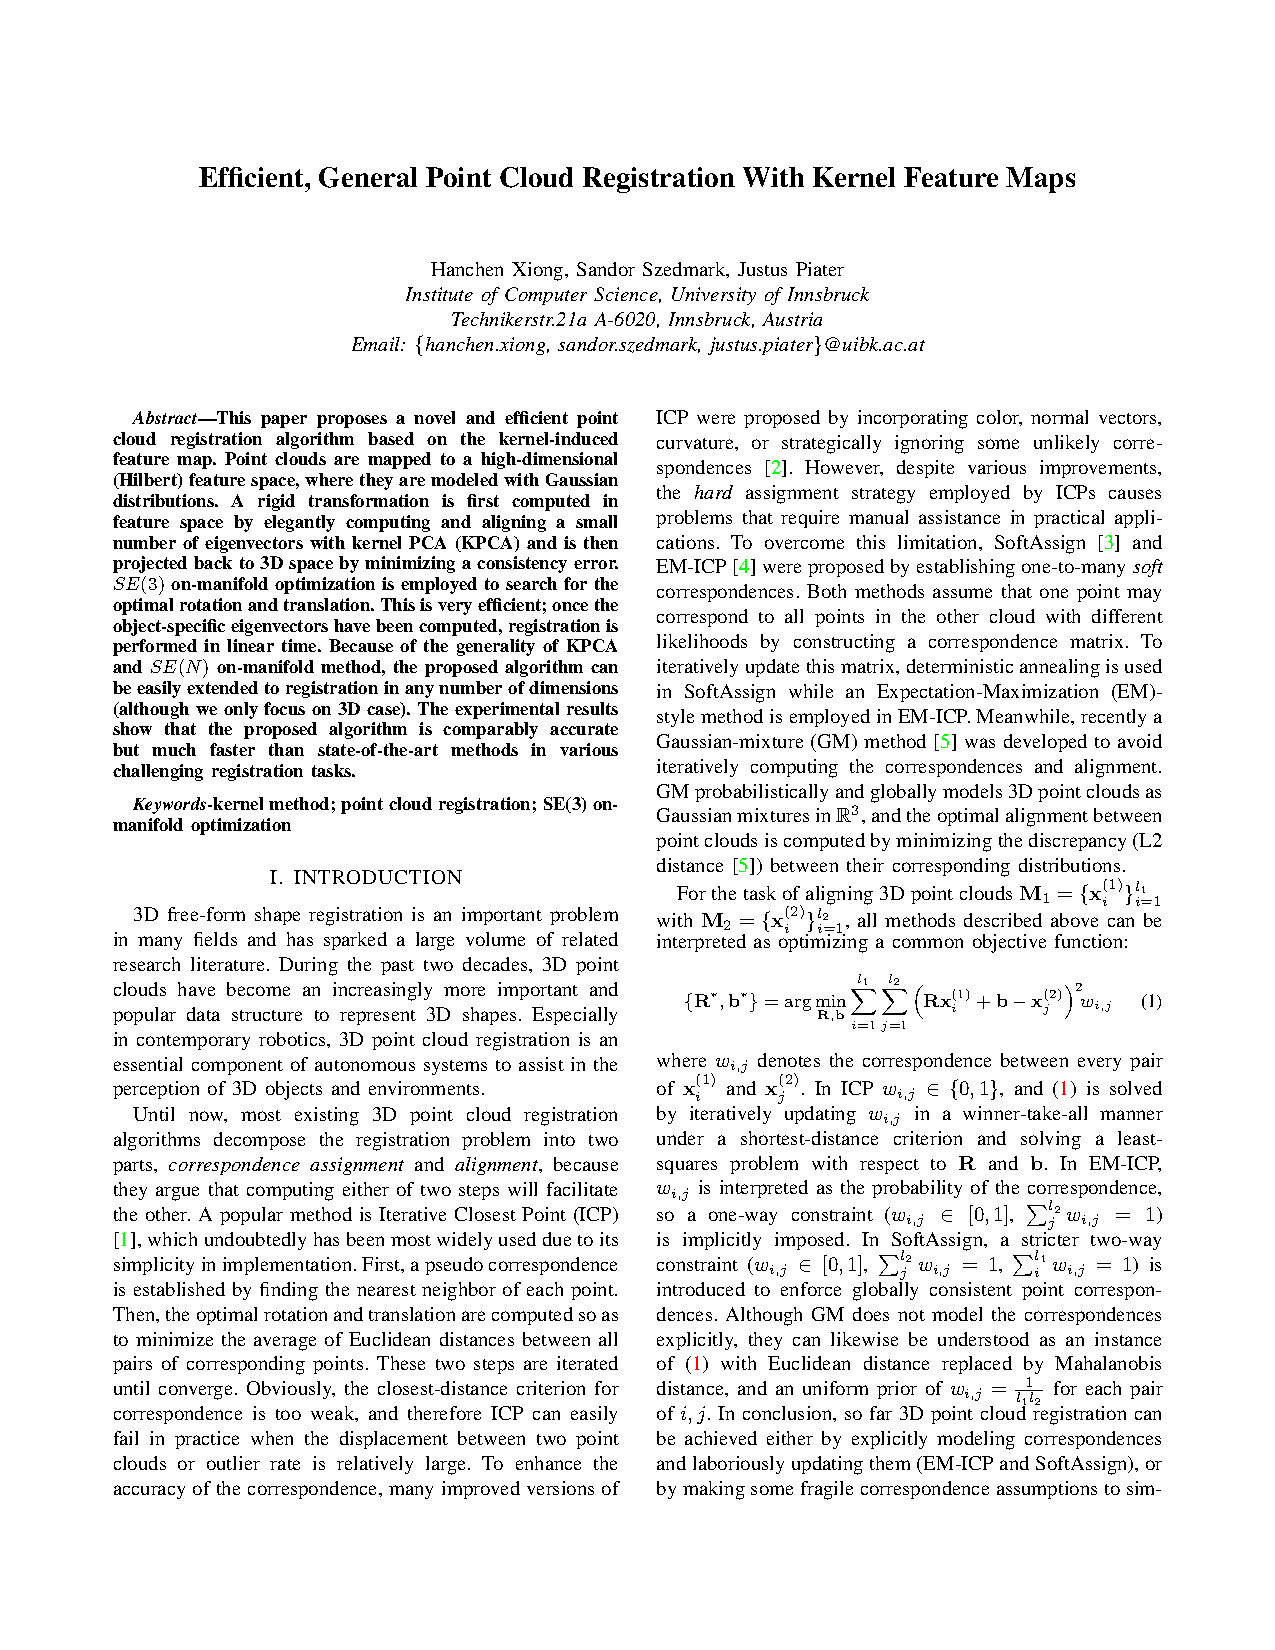
\includepdf[offset=3cm -3cm, scale=1, pages=-,pagecommand={\pagestyle{fancy}}]{./Papers/Xiong-2013-CRV.pdf}



%----------------------------------------------------------------------------------------
%	SECTION 2
%----------------------------------------------------------------------------------------



%\section{Stochastic Optmization of Black-box Functions on Riemannian Manifolds using Kernel Adaptive Sequential Monte Carlo}
%
%Sed ullamcorper quam eu nisl interdum at interdum enim egestas. Aliquam placerat justo sed lectus lobortis ut porta nisl porttitor. Vestibulum mi dolor, lacinia molestie gravida at, tempus vitae ligula. Donec eget quam sapien, in viverra eros. Donec pellentesque justo a massa fringilla non vestibulum metus vestibulum. Vestibulum in orci quis felis tempor lacinia. Vivamus ornare ultrices facilisis. Ut hendrerit volutpat vulputate. Morbi condimentum venenatis augue, id porta ipsum vulputate in. Curabitur luctus tempus justo. Vestibulum risus lectus, adipiscing nec condimentum quis, condimentum nec nisl. Aliquam dictum sagittis velit sed iaculis. Morbi tristique augue sit amet nulla pulvinar id facilisis ligula mollis. Nam elit libero, tincidunt ut aliquam at, molestie in quam. Aenean rhoncus vehicula hendrerit.
%
%
%
